%=====================================================================
%  SHARED PREAMBLE — Quantitative Reasoning LAB 413 Beamer theme
%  Paste this block VERBATIM at the top of every LabN_beamer.tex
%  (keep each deck self-contained; do NOT \input this file).
%  Compile: pdflatex LabN_beamer.tex   (run twice for footline counters)
%=====================================================================
\documentclass[aspectratio=169,11pt]{beamer}

\usepackage[utf8]{inputenc}
\usepackage[T1]{fontenc}
\usepackage{lmodern}
\usepackage{amsmath,amssymb}
\usepackage{graphicx}
\usepackage{booktabs}
\usepackage{tcolorbox}
\tcbuselibrary{skins}

\usetheme{default}
\usecolortheme{default}
\useinnertheme{circles}

\definecolor{qrnavy}{RGB}{20,44,90}
\definecolor{qrblue}{RGB}{38,80,150}
\definecolor{qrgray}{RGB}{90,95,105}
\definecolor{qrlight}{RGB}{234,239,247}
\definecolor{qrred}{RGB}{190,60,60}

\setbeamercolor{structure}{fg=qrnavy}
\setbeamercolor{frametitle}{fg=white,bg=qrnavy}
\setbeamercolor{title}{fg=qrnavy}
\setbeamercolor{block title}{fg=white,bg=qrblue}
\setbeamercolor{block body}{bg=qrlight}
\setbeamercolor{itemize item}{fg=qrblue}
\setbeamercolor{itemize subitem}{fg=qrblue}
\setbeamerfont{frametitle}{series=\bfseries}
\setbeamertemplate{navigation symbols}{}

\setbeamertemplate{frametitle}{%
  \nointerlineskip
  \begin{beamercolorbox}[wd=\paperwidth,ht=3.2ex,dp=1.2ex,leftskip=0.3cm]{frametitle}%
    \strut\insertframetitle\strut
  \end{beamercolorbox}%
}

% Footline: course | lab N | slide number  (edit "Lab N" per deck)
\newcommand{\labnum}{Lab 3}   % <-- SET THIS to the lab number, e.g. \renewcommand{\labnum}{Lab 3}
\setbeamertemplate{footline}{%
  \leavevmode%
  \hbox{%
    \begin{beamercolorbox}[wd=.5\paperwidth,ht=2.4ex,dp=1ex,leftskip=.3cm]{author in head/foot}%
      \usebeamerfont{author in head/foot}\color{qrgray}\small Quantitative Reasoning -- LAB 413%
    \end{beamercolorbox}%
    \begin{beamercolorbox}[wd=.5\paperwidth,ht=2.4ex,dp=1ex,rightskip=.3cm]{title in head/foot}%
      \usebeamerfont{title in head/foot}\color{qrgray}\small\hfill \labnum \quad\insertframenumber\,/\,\inserttotalframenumber%
    \end{beamercolorbox}}%
}

% Number badge (01, 02, ...) used on concept slides:  \numbadge{01}
\newtcbox{\numbadge}{on line,boxsep=2pt,left=4pt,right=4pt,top=2pt,bottom=2pt,
  colback=qrnavy,colframe=qrnavy,fontupper=\bfseries\color{white},arc=2pt}

% Key-concepts callout:  \begin{keybox} ... \end{keybox}   or  \begin{keybox}[Scenario] ...
\newtcolorbox{keybox}[1][Key Concepts]{colback=qrlight,colframe=qrnavy,
  fonttitle=\bfseries,title={#1},coltitle=white,arc=2pt,left=4pt,right=4pt,
  top=3pt,bottom=3pt,boxrule=0.6pt}

%---------------------------------------------------------------------
%  Title data
%---------------------------------------------------------------------
\title{\bfseries Regression \& Residuals}
\subtitle{Week 4 Recap \textbullet\ Lab 3}
\author{Instructor: Subin Na}
\institute{Quantitative Reasoning -- LAB 413}
\date{September 17, 2025}

\begin{document}

%---------------------------------------------------------------------
%  Title slide
%---------------------------------------------------------------------
{\setbeamertemplate{footline}{}
\begin{frame}
  \vfill
  {\color{qrgray}\small Quantitative Reasoning -- LAB 413}\\[0.6em]
  {\usebeamerfont{title}\color{qrnavy}\huge\bfseries Regression \& Residuals\par}
  \vspace{0.4em}
  {\color{qrblue}\large Week 4 Recap \ \textbullet\ \ Lab 3}\par
  \vspace{1.6em}
  {\color{qrgray} Instructor: \textbf{Subin Na} \hfill September 17, 2025}
  \vfill
\end{frame}
}

%---------------------------------------------------------------------
%  Today's Plan
%---------------------------------------------------------------------
\begin{frame}{Today's Plan}
  \begin{columns}[T]
    \begin{column}{0.5\textwidth}
      \textbf{\color{qrnavy}1. Quick Recap}
      \begin{itemize}
        \item Regression \& Residuals
        \item Hands-on Practice --- fitting regression lines in R
        \item Exploring Residuals --- plots \& interpretation
        \item Cautions in Regression --- outliers, extrapolation, omitted variables
      \end{itemize}
    \end{column}
    \begin{column}{0.5\textwidth}
      \phantom{\textbf{x}}
      \vspace{2.2em}

      \textbf{\color{qrnavy}2. RStudio Practice}
    \end{column}
  \end{columns}
\end{frame}

%---------------------------------------------------------------------
%  01 Regression Basics
%---------------------------------------------------------------------
\begin{frame}{\numbadge{01}\ \ Regression Basics}
  \begin{keybox}
    Draw the best-fitting line through the data to predict $Y$ from $X$.
  \end{keybox}
  \vspace{0.3em}
  \begin{equation*}
    Y_i \;=\; \underbrace{\alpha}_{\text{intercept}}
      \;+\; \underbrace{\beta}_{\text{slope}}\cdot X_i
      \;+\; \underbrace{\epsilon_i}_{\text{error term}}
  \end{equation*}
  \vspace{-0.2em}
  \begin{columns}[T]
    \begin{column}{0.5\textwidth}
      \small
      \begin{itemize}
        \item \textbf{Intercept ($\alpha$):} value of $Y$ when $X = 0$ (starting point).
        \item \textbf{Slope ($\beta$):} change in $Y$ per one-unit change in $X$.
        \item \textbf{Residuals:} prediction errors.
      \end{itemize}
    \end{column}
    \begin{column}{0.5\textwidth}
      \centering
      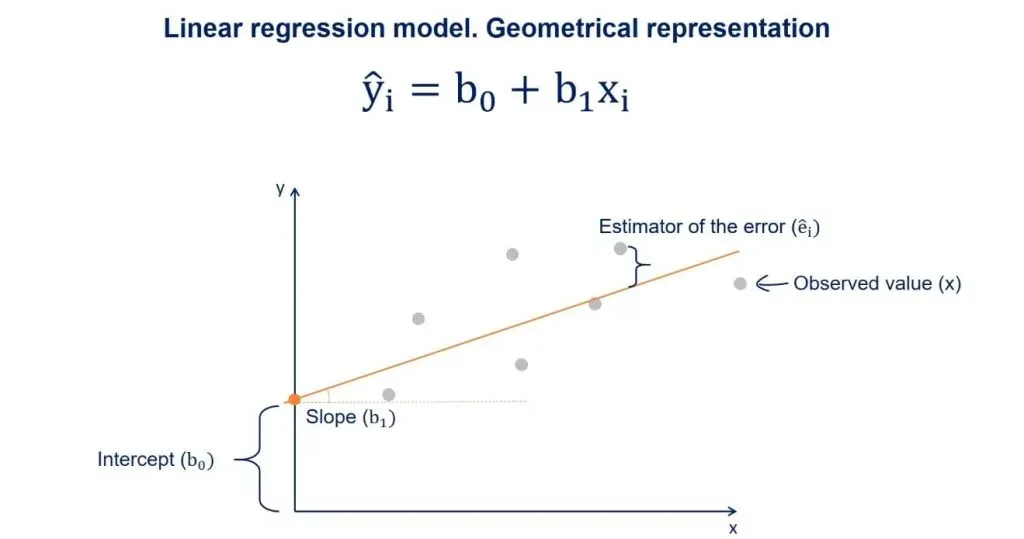
\includegraphics[width=\textwidth]{figures/s03_2_9.7x5.2.png}
    \end{column}
  \end{columns}
\end{frame}

%---------------------------------------------------------------------
%  02 Least Squares Regression  (EMBED scatter)
%---------------------------------------------------------------------
\begin{frame}{\numbadge{02}\ \ Least Squares Regression}
  \begin{columns}[T]
    \begin{column}{0.46\textwidth}
      \begin{keybox}
        The best-fit line \textbf{minimizes} the vertical distances between the
        points and the line.
      \end{keybox}
      \vspace{0.4em}
      \begin{itemize}
        \item We minimize the \textbf{Sum of Squared Residuals (SSR)}.
        \item The regression line is the one with the \textbf{smallest total error}.
      \end{itemize}
    \end{column}
    \begin{column}{0.54\textwidth}
      \centering
      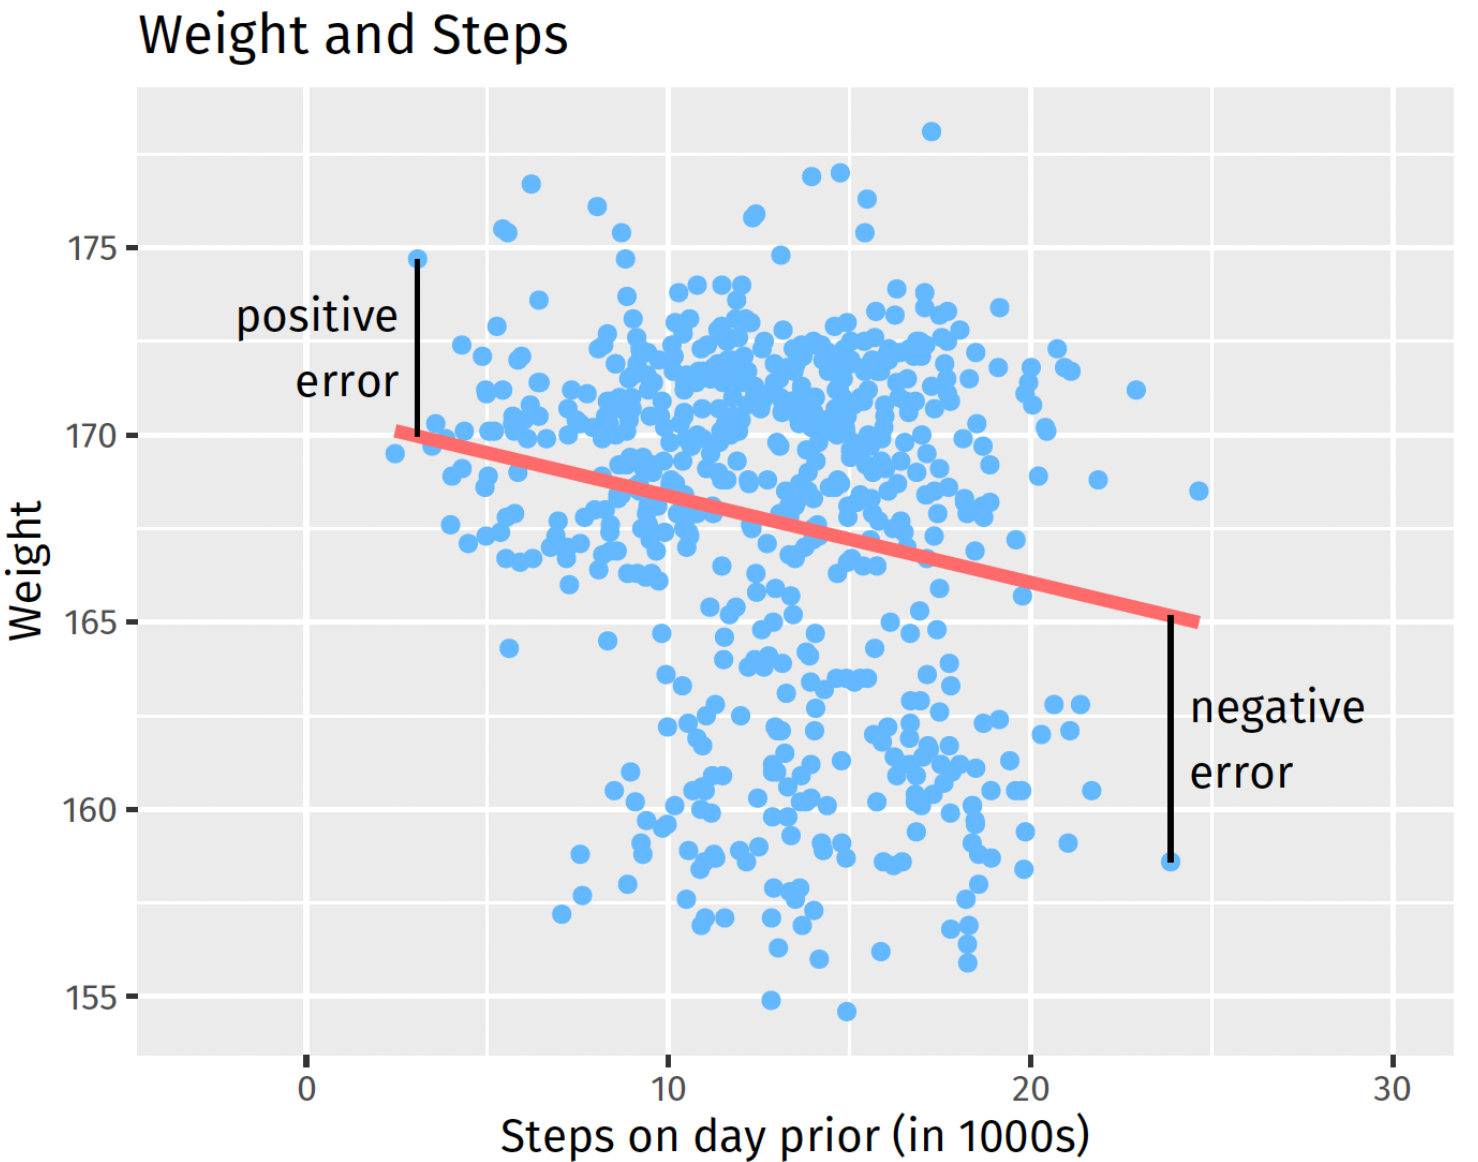
\includegraphics[width=\textwidth]{figures/s04_1_8.1x6.3.png}
    \end{column}
  \end{columns}
\end{frame}

%---------------------------------------------------------------------
%  03 Residuals  (EMBED scatter)
%---------------------------------------------------------------------
\begin{frame}{\numbadge{03}\ \ Residuals}
  \begin{columns}[T]
    \begin{column}{0.46\textwidth}
      \begin{keybox}
        Residual $=$ actual $Y$ $-$ predicted $Y$.
      \end{keybox}
      \vspace{0.4em}
      \begin{itemize}
        \item Show how far the data deviate from the regression line.
        \item Average of residuals $= 0$ (a special property of the least-squares line).
      \end{itemize}
    \end{column}
    \begin{column}{0.54\textwidth}
      \centering
      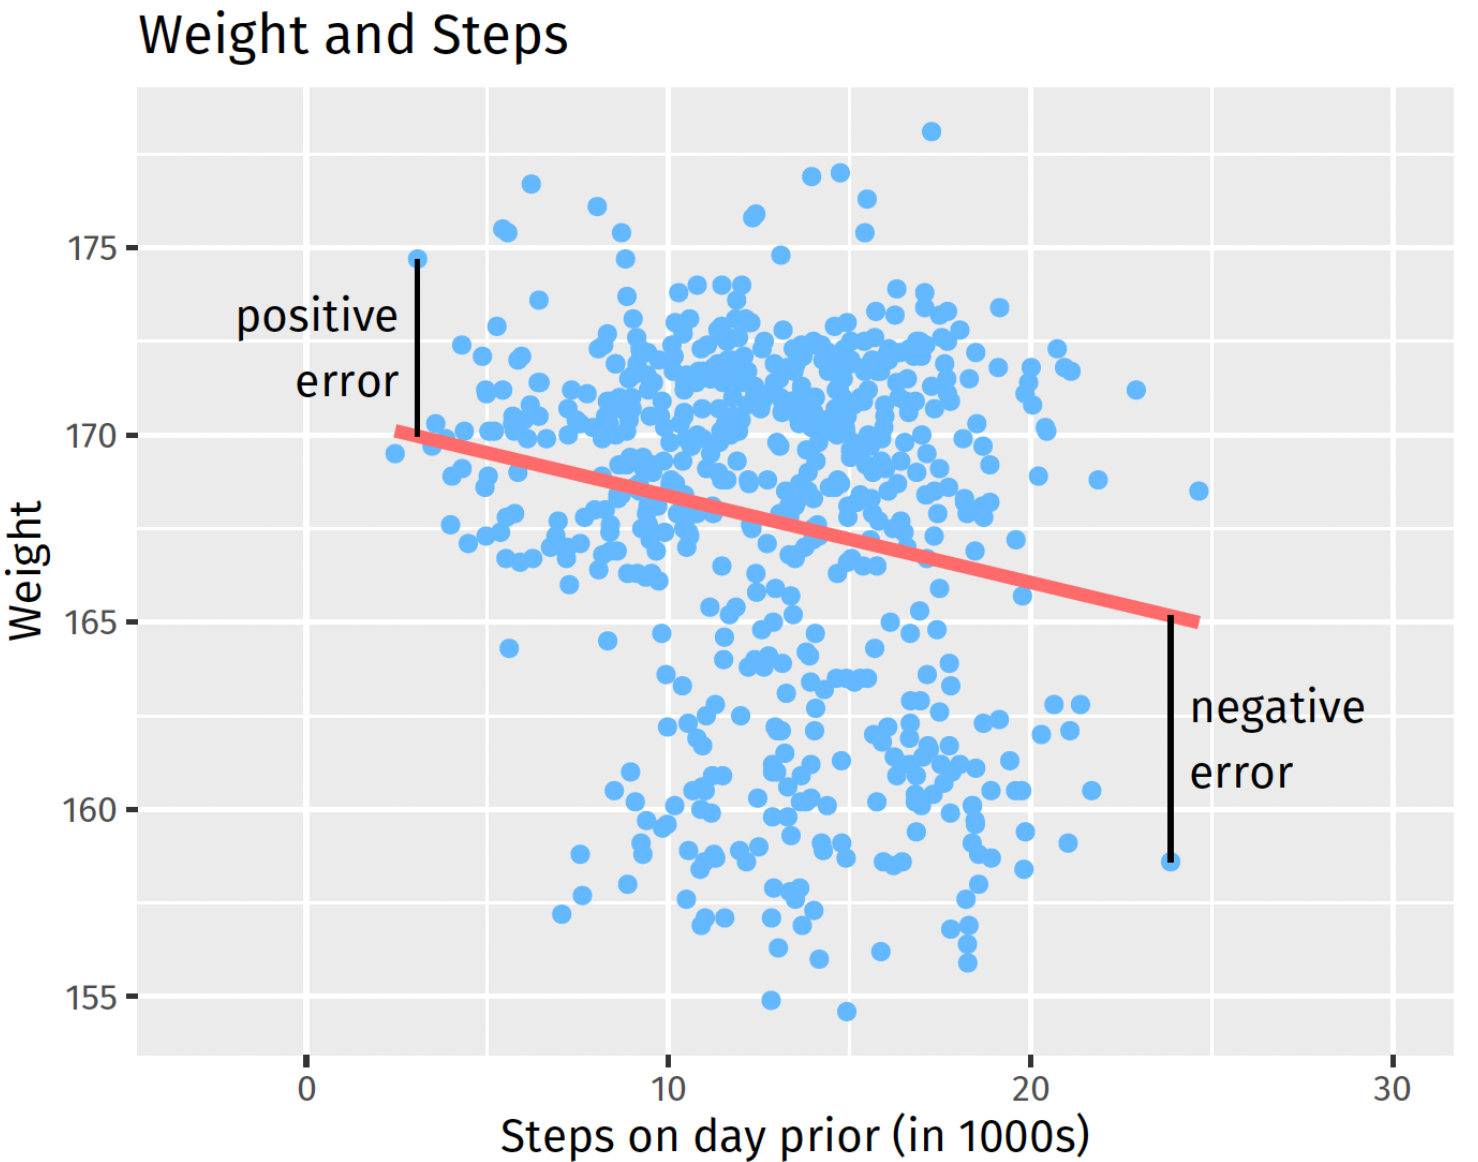
\includegraphics[width=\textwidth]{figures/s05_1_5.7x4.5.png}
    \end{column}
  \end{columns}
\end{frame}

%---------------------------------------------------------------------
%  04 R-Squared
%---------------------------------------------------------------------
\begin{frame}{\numbadge{04}\ \ R-Squared}
  \begin{keybox}
    $R^2$ measures the proportion of variance in $Y$ that is \textbf{explained} by $X$.
  \end{keybox}
  \vspace{0.6em}
  \begin{itemize}
    \item Ranges from $0$ to $1$: closer to $1$ means the line explains more of the
          variation in $Y$.
    \item Closer to $0$ means the predictor $X$ explains little of the variation.
  \end{itemize}
\end{frame}

%---------------------------------------------------------------------
%  05 Cautions (1)  (EMBED interpolation vs extrapolation)
%---------------------------------------------------------------------
\begin{frame}{\numbadge{05}\ \ Cautions (1)}
  \begin{keybox}
    \begin{itemize}
      \item \textbf{Outliers} can strongly affect a regression.
      \item Avoid \textbf{extrapolation} --- predicting far outside the data range.
    \end{itemize}
  \end{keybox}
  \vspace{0.4em}
  \begin{center}
    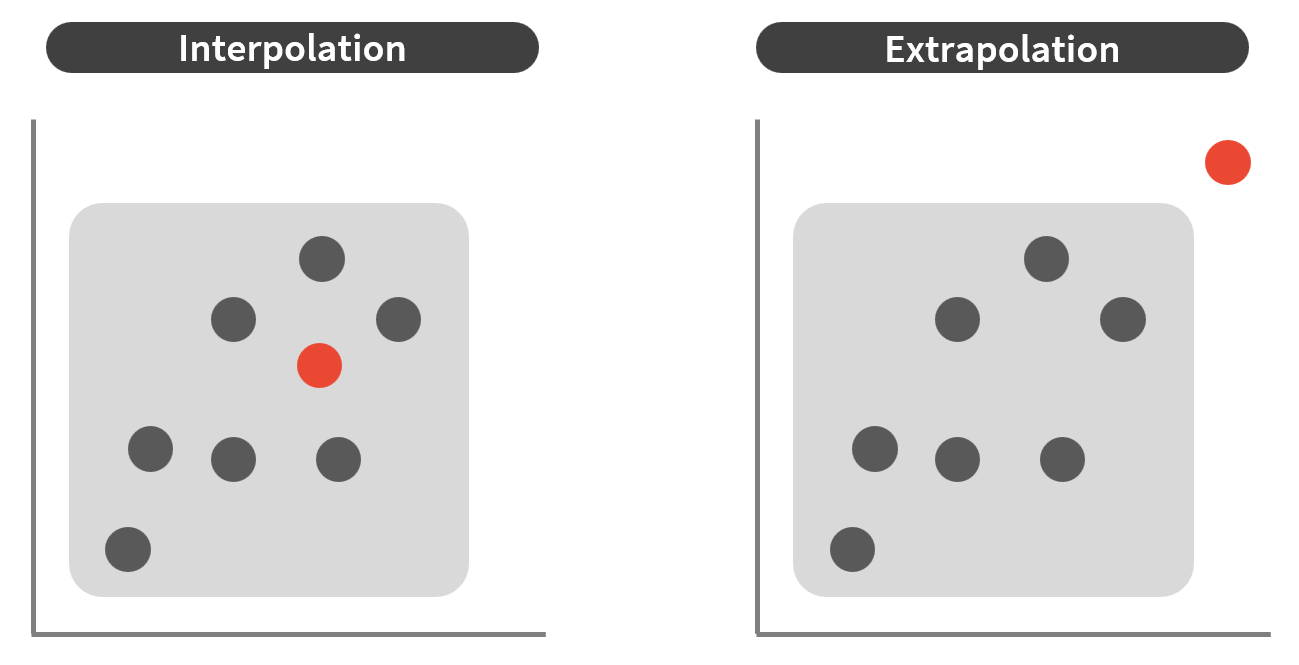
\includegraphics[width=0.78\textwidth]{figures/s07_1_9.0x4.6.png}
  \end{center}
\end{frame}

%---------------------------------------------------------------------
%  05 Cautions (2)
%---------------------------------------------------------------------
\begin{frame}{\numbadge{05}\ \ Cautions (2)}
  \begin{keybox}
    \begin{itemize}
      \item Beware of \textbf{omitted variables}.
      \item \textbf{Simpson's paradox:} when the trend in the whole dataset is the
            \emph{opposite} of the trend within the smaller groups that make it up.
    \end{itemize}
  \end{keybox}
  \vspace{0.8em}
  \begin{center}
    {\large\bfseries\color{qrred} Remember: correlation $\neq$ causation}
  \end{center}
\end{frame}

%---------------------------------------------------------------------
%  Transition to RStudio
%---------------------------------------------------------------------
{\setbeamertemplate{footline}{}
\begin{frame}
  \vfill
  \centering
  {\color{qrnavy}\Huge\bfseries RStudio Practice}\\[0.8em]
  {\color{qrblue}\large Correlation, Regression \& Residuals in R}\\[0.4em]
  {\color{qrgray} See \texttt{Lab3.Rmd} / \texttt{lab3\_master file.R}}
  \vfill
\end{frame}
}

\end{document}
